\section[Equation consistency in electron-only reconnection manuscripts]{\raggedright Equation consistency in electron-only reconnection
manuscripts}\label{equation-consistency-in-electron-only-reconnection-manuscripts}

\textbf{Taylor Kalin}\\
\url{https://taylorkalin.com} ;
\href{mailto:teylersf@gmail.com}{\nolinkurl{teylersf@gmail.com}}\\
ORCID: \url{https://orcid.org/0009-0003-9000-9315}\\
Version 1.0.0; 29 October 2026

\subsection{Abstract}\label{abstract}

We check the equations in Liu et al.'s arXiv:2407.06020v2, its
publisher-hosted accepted manuscript, and the supplement embedded in
that arXiv version. The inspected main system has a continuity sign and
a dimensional pressure coefficient inconsistent with its stated Appendix
rewrite. After restoring the pressure coefficient, the printed
continuity sign gives growing rather than oscillatory linear modes.
Separately, the supplemental density-energy term lacks the one-half
coefficient required by its claimed quadratic invariant. An exact
periodic state demonstrates nonconservation of that printed sum while
the consistently weighted sum is conserved. Direct Gaussian projection
also gives collisionless Hermite streaming and forcing signs opposite to
those printed in the supplied hierarchy. These repairs reconcile the
displays with the established KREHM equations; they do not introduce a
new plasma model. The source's reconnection-rate and conditional
coalescence scalings retain their algebraic support. The subscription
version of record and final journal supplement were not obtained, and no
conclusion about the actual solver or numerical curves follows from
these consistency tests.

\subsection{1. Editions and purpose}\label{editions-and-purpose}

Liu, Silva, Milanese, Zhou, Mandell and Loureiro study electron-only
reconnection and inverse magnetic-energy transfer {[}1{]}. We read the
complete supplied 19-page arXiv:2407.06020v2, including its ten appended
supplemental pages, and the authentic ten-page CHORUS accepted
manuscript openly linked by APS. The latter contains a cover and nine
manuscript pages dated 19 March 2025. It retains the main governing
displays and Appendix considered here, while correcting a Figure 1
decimal, consolidating supplement references and changing pagination.
The supplied file is byte-identical to official arXiv v2, posted 10
March and dated 11 March 2025.

The associated journal article is Physical Review Letters 134, 155201,
DOI 10.1103/PhysRevLett.134.155201. Its subscription version of record
was not obtained. The accepted manuscript is a distinct edition; its
cover does not establish identity with the typeset article. Supplemental
findings below concern specifically arXiv v2, whose supplement is absent
from the accepted-manuscript file. We therefore make an edition-specific
consistency claim, not a claim that these defects remain in the
uninspected journal copies.

The distinctions matter. Appendix A already contains a core sign and
coefficient consistent with the original KREHM framework {[}2{]}. Its
reconnection calculation uses magnitudes and can remain valid despite
transcription defects in earlier displays. Our contribution is to
document the internal differences and supply reproducible identities
that a literal implementation can check. The standard model, energy and
Hermite representation belong to the cited prior theory {[}2,3{]}.

\subsection{2. Main system and its Appendix
reduction}\label{main-system-and-its-appendix-reduction}

Use the stated positive elementary charge and conventions

\[
\begin{aligned}
N&=\frac{\delta n_e}{n_0},&
D_t&=\partial_t+\frac c{B_0}\{\varphi,\cdot\},\\
\mathcal D_\parallel&=\partial_z-\frac1{B_0}\{A,\cdot\},&
u&=\frac{ed_e^2}{cm_e}\Delta_\perp A.
\end{aligned}
\tag{1}
\]

where \(\{f,g\}=f_xg_y-f_yg_x\), \(A=A_z=A_\parallel\), and
\(d_e^2=c^2m_e/(4\pi n_0e^2)\). The main article's Eqs. (1) and (2) are
on arXiv page 1 and accepted-manuscript printed page 1, PDF page 2. The
coefficient-consistent, isothermal, collisionless system is

\[
\begin{aligned}
D_tN&=-\mathcal D_\parallel u,\\
D_t(A-d_e^2\Delta_\perp A)
&=-c\partial_z\varphi+\frac{cT_e}{e}\mathcal D_\parallel N.
\end{aligned}
\tag{2}
\]

KREHM Eqs. (39) and (40) give these signs and the pressure coefficient
under the same conventions {[}2{]}. The inspected main Eq. (1) instead
prints a positive parallel derivative of \(u\), and its Eq. (2) omits
\(cT_e/e\) in front of the density gradient. A bare \(\nabla N\) has
inverse-length dimensions; it cannot be added to \(\partial_tA\) in the
dimensional notation being used. An explicitly declared normalization
could set a coefficient to one numerically, but would have to transform
the other factors and the claimed Appendix rewrite consistently.

For \(\partial_z=0\), Eq. (2) gives

\[
\partial_tN+\frac c{B_0}\{\varphi,N\}
=\frac{ed_e^2}{cm_eB_0}\{A,\Delta_\perp A\}.
\tag{3}
\]

This is the positive bracket printed in Appendix (A1), arXiv page 5 and
accepted-manuscript PDF page 6. Direct reduction of the printed positive
main parallel derivative instead gives a negative bracket. Changing
\(A_\parallel\) to \(-A_z\) cannot repair this quadratic term because
\(\{-A,\Delta(-A)\}=\{A,\Delta A\}\). Appendix (A2) also restores the
missing pressure coefficient. A positive parallel derivative does occur
in KREHM summary Eq. (62), but there it evolves a polarization variable
equal to minus the density perturbation {[}2{]}. That change of
dependent variable must be retained.

The linear check isolates the sign after restoring the pressure units.
For a perpendicular Fourier symbol \(0\le\Gamma_0<1\), Poisson closure
gives \(\varphi=-T_iN/[e(1-\Gamma_0)]\). About a uniform guide field,
the consistently signed pair has

\[
\omega^2=
\frac{k_\parallel^2d_e^2k_\perp^2}
 {m_e(1+d_e^2k_\perp^2)}
\left(T_e+\frac{T_i}{1-\Gamma_0}\right)>0.
\tag{4}
\]

The printed continuity sign gives the opposite frequency squared,
equivalently positive real time-growth eigenvalues. Figure 1 illustrates
the isolated contrast. It is not an instability observed in the source's
simulation. A plausible explanation is that the implementation uses the
established equations while the displays contain transcription defects.

\subsection{3. The density coefficient in the energy
invariant}\label{the-density-coefficient-in-the-energy-invariant}

Supplement Eq. (12), supplemental page 8 or combined arXiv page 17,
prints \(Y_{\rm p}=n_0T_e\langle N^2\rangle\) and writes
\(U+K_i+K_e+Y_{\rm p}\) as a conserved free energy. Its other terms
retain their usual coefficients. Let brackets denote a periodic volume
mean. In the strict-subion closure \(\varphi=-T_iN/e\), the consistent
terms are

\[
\begin{aligned}
U&=\frac{\langle|\nabla_\perp A|^2\rangle}{8\pi},&
K_e&=\frac{d_e^2\langle(\Delta_\perp A)^2\rangle}{8\pi},\\
K_i&=\frac{n_0T_i}{2}\langle N^2\rangle,&
Y_{1/2}&=\frac{n_0T_e}{2}\langle N^2\rangle.
\end{aligned}
\tag{5}
\]

The one-half density coefficient is also explicit in KREHM Eqs.
(70)--(71) {[}2{]}. We interpret the source's finite-FLR ion term in its
usual self-adjoint quadratic-form sense, not as an operator acting on an
already squared field. In the subion limit its printed definitions imply
\(K_i/Y_{\rm p}=T_i/(2T_e)\). At equal temperatures this is one half,
whereas the following supplemental explanation invokes \(K_i\approx Y\).
The consistent density coefficient yields \(K_i/Y_{1/2}=T_i/T_e\).

Conservation supplies a stronger test than that ratio. For the
two-dimensional periodic Appendix system (\(\partial_z=0\)), write
\(F=A-d_e^2\Delta A\), \(\alpha=ed_e^2/(cm_eB_0)\) and
\(I=\langle N\{A,\Delta A\}\rangle\). Retain the full Appendix advection
of \(F\), including its inertial part. Periodic integration by parts
then gives

\[
\frac{d(U+K_e)}{dt}=-n_0\alpha(T_i+T_e)I,\qquad
\dot K_i=n_0\alpha T_i I,\qquad
\dot Y_{1/2}=n_0\alpha T_e I.
\tag{6}
\]

In particular, \(\langle\Delta A\{\Delta A,N\}\rangle=0\) cancels the
integrated inertial-advection contribution; the inertial-advection field
itself need not vanish. Equation (6) conserves \(U+K_e+K_i+Y_{1/2}\),
but replacing only \(Y_{1/2}\) by \(Y_{\rm p}=2Y_{1/2}\) leaves
\(n_0\alpha T_e I\). The density variance is not separately invariant
for general coupled states, so a change in its diagnostic name cannot
repair the unweighted sum.

An exact periodic witness on \([0,2\pi]^2\) is

\[
\begin{aligned}
A&=\cos x+\cos2y,& N&=\sin x\sin2y,\\
\{A,\Delta A\}&=-6\sin x\sin2y,& I&=-\frac32.
\end{aligned}
\tag{7}
\]

The unit-amplitude fields specify an algebraic normalization. Scaling
both by any \(0<\epsilon<1\) makes the density \(n_0(1+\epsilon N)\)
positive and the fluctuations arbitrarily small; \(I\) and the nonzero
energy residual scale as \(\epsilon^3\). Thus the discrepancy does not
depend on using order-one density perturbations.

Choose coherent nondimensional coefficients \(G=1\), \(\kappa=1\),
\(n_0=\alpha=1\), \(T_e=T_i=1\), \(d_e^2=1/4\), where the magnetic
energy is \(G/2\) times its quadratic form and \(G\kappa=n_0\alpha\).
Exact inversion of \(1-d_e^2\Delta\) gives

\[
\begin{aligned}
(\dot U,\dot K_e,\dot K_i,\dot Y_{1/2})
&=\left(\frac{21}{20},\frac{39}{20},-\frac32,-\frac32\right),\\
\dot W_{1/2}&=0,\qquad \dot W_{\rm p}=-\frac32.
\end{aligned}
\tag{8}
\]

These are instantaneous derivatives of a synthetic admissible state, not
a time integration or a measured heating rate. Figure 8 of the source
could already use the consistent coefficient; its raw arrays and
implementation were not obtained. Neither that figure nor the
order-of-magnitude equipartition assumption is rejected by this test.

\begin{minipage}{\linewidth}
\pandocbounded{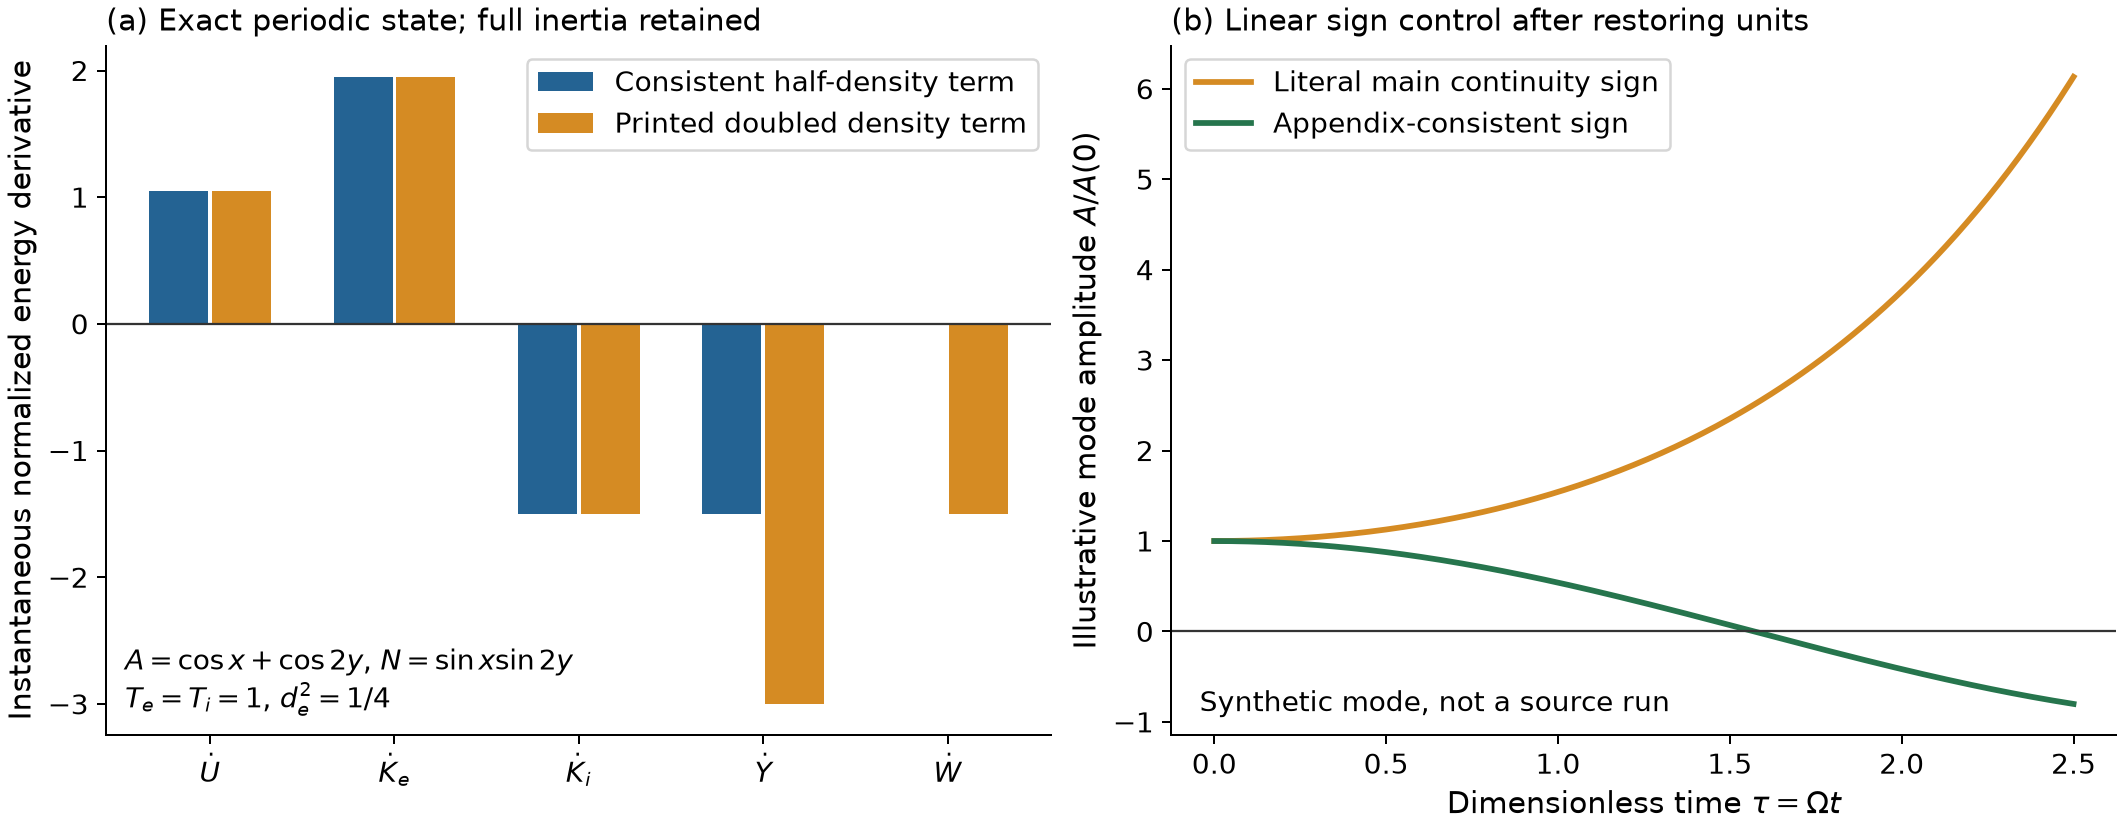
\includegraphics[keepaspectratio]{images/energy-and-wave-controls.png}}

Figure 1. Left: the exact ledger of Eq. (8), retaining full inertia,
compared with changing only the density coefficient. Right: the
unit-frequency linear control \(A/A(0)=\cos\tau\) or \(\cosh\tau\) after
restoring the pressure coefficient, with initial amplitude one and
initial derivative zero. Both panels are synthetic equation checks;
neither reproduces a source run.
\end{minipage}

\subsection{4. Collisionless Hermite
projection}\label{collisionless-hermite-projection}

Supplement Eq. (9), combined page 15, uses \(F_0\propto e^{-z^2}\),
\(z=v_\parallel/v_{\rm the}\), and the expansion
\(\psi_m=H_m/\sqrt{2^m m!}\). Its drive is
\((1-2z^2)F_0\mathcal D_\parallel u\). The stated physicists' Hermite
convention fixes

\[
H_2=4z^2-2,\qquad
1-2z^2=-\sqrt2\,\psi_2,\qquad
\langle H_2(1-2z^2)\rangle_{F_0}=-4,
\quad \langle H_2^2\rangle_{F_0}=8.
\tag{9}
\]

Thus the projected \(g_2\) drive is negative
\(\sqrt2\mathcal D_\parallel u\), while supplement Eq. (11) prints a
positive sign. In the two-dimensional case used for its non-isothermal
experiment, Eq. (9)'s left-hand streaming term is
\(+v_\parallel\mathcal D_\parallel(g-\theta F_0)\), where
\(\theta=\delta T_{\parallel e}/T_e\). With collisions set to zero,
projection gives

\[
D_tg_m=-v_{\rm the}\mathcal D_\parallel
\left(\sqrt{\frac{m+1}{2}}g_{m+1}
+\sqrt{\frac m2}g_{m-1}-\delta_{m1}g_2\right)
-\sqrt2\,\delta_{m2}\mathcal D_\parallel u,
\qquad m\ge2.
\tag{10}
\]

The printed hierarchy instead has positive streaming on its right-hand
side. KREHM Eq. (93) independently corroborates Eq. (10) {[}2{]}. For
example, the \(g_2\leftarrow g_3\) coefficient on that side is
\(-\sqrt{3/2}\) and the temperature moment obeys
\(D_t\theta+\sqrt3v_{\rm the}\mathcal D_\parallel g_3=-2\mathcal D_\parallel u\).

Reversing the velocity coordinate rephases odd Hermite coefficients but
leaves the even \(m=2\) forcing unchanged. A redefinition that changes
this forcing must also change the supplied distribution expansion and
temperature moment. These silent changes do not make the two stated
equations identical. Figure 2 shows the direct Gaussian identities. We
assign no sign to the separately written collision functional; the
contradiction already exists without collisions. Reversing a streaming
matrix alone also does not establish failed Landau damping in an
uninspected implementation.

\begin{minipage}{\linewidth}
\pandocbounded{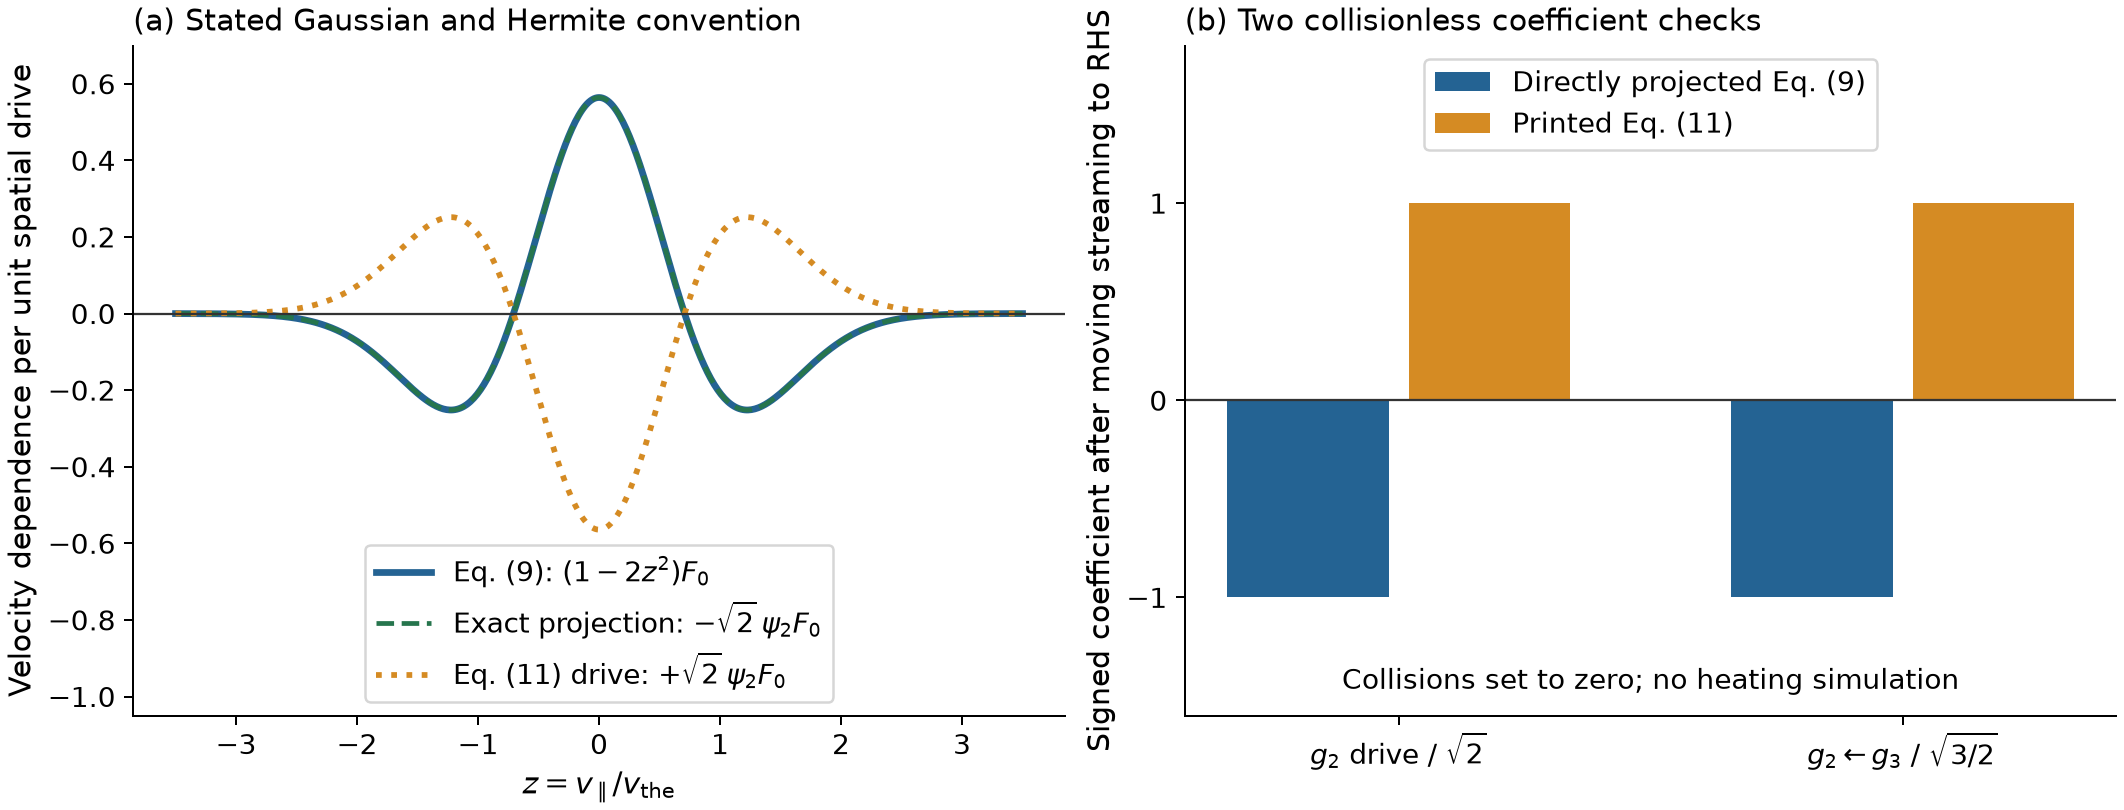
\includegraphics[keepaspectratio]{images/hermite-projection-controls.png}}

Figure 2. Left: the source in Eq. (9) and its exact negative-\(\sqrt2\)
Hermite representation overlap; the positive representation has the
opposite sign. Right: two signed coefficients after moving streaming to
the right-hand side. Collisions are zero, and no heating simulation is
supplied.
\end{minipage}

\subsection{5. Retained physics and additional presentation
limits}\label{retained-physics-and-additional-presentation-limits}

Using the consistent Appendix coefficients and the source assumptions
\(\delta_x\sim d_e\), \(\delta_y\sim R\) and
\(A_{\rm sheet}\sim B_\perp d_e\) retains

\[
\tau_{\rm rec}\sim\frac R{d_e}\tau,\qquad
\mathcal R_{\rm rec}\sim\sqrt{1+T_i/T_e}\frac{\rho_s}{R},
\qquad \mathcal R_{{\rm rec},e}\sim\frac{d_e}{R}.
\tag{11}
\]

The last two rates use different normalizing velocities. Exceeding a
familiar ion-Alfvén-normalized value is not by itself an impossible
outflow-normalized rate. Conserved island flux \(RB_\perp\), volume
filling and a merger-controlled lifetime imply
\(\tau_{\rm rec}\propto R^2/B_\perp\) and therefore

\[
\mathcal E\propto t^{-2/3},\qquad R\propto t^{1/3},\qquad
B_\perp\propto t^{-1/3},\qquad l\propto t^{2/3}
\tag{12}
\]

with the source's critical-balance assumption for \(l\). The
constant-rate MHD algebra likewise retains \(\mathcal E\propto t^{-1}\)
and \(R\propto t^{1/2}\). These are conditional phenomenological
deductions; our checks neither refit nor disprove the source's
finite-window numerical evidence.

Two subsidiary dimensional displays need clarification. The v2
supplement defines ion beta as \(4\pi n_{0i}m_i/B_0^2\), an inverse
velocity squared in dimensional Gaussian units. The conventional
dimensionless definition is \(8\pi n_{0i}T_i/B_0^2\) {[}3{]}. Its
supplemental Eq. (4) also leaves the combined parallel density
derivative without the coefficient \(c(T_e+T_i)/e\). These can be
documented as presentation inconsistencies without inferring the
numerical units used by a solver.

With conventional beta, the supplement's proposed finite-beta rate, with
its entire fraction inside the square root, matches the ERMHD
coefficient and has the correct common low-beta limit {[}3{]}. The
source explicitly acknowledges that ideal ERMHD omits flux-breaking
physics and labels this extension a hypothesis requiring validation. We
retain that admission rather than presenting it as an overlooked defect.

The supplemental length-definition prose reverses the parallel and
perpendicular contour-intercept assignments, but the figure axes and
reported length scale do not establish that the actual diagnostic was
reversed. Overall constants in its normalized structure function and
unit local-field direction cancel and are not additional failures. The
supplied shell-advection maps, spectral-peak motion and size growth
remain relevant positive observations. Original fields would be needed
to remeasure a complete energy-transfer budget.

\subsection{6. Reproduction, conclusions and
availability}\label{reproduction-conclusions-and-availability}

The original producer {[}5{]} uses full finite Fourier convolution and
rational arithmetic, without spectral truncation. For
\(A=a\cos(mx)+b\cos(ny)\) and \(N=h\sin(mx)\sin(ny)\) it checks
\(I=habmn(m^2-n^2)/4\). Five patterns
\((m,n,a,b,h)=(1,2,1,1,1),(2,3,1/2,2,-1),(3,1,2,1/3,3/2),(1,1,1,1,1),(1,2,0,1,1)\)
cross four \((T_e,T_i)=(1,1),(1/2,2),(3,1/3),(2,3)\) and three
\(d_e^2=0,1/4,2\). These give 60 states, including 24 zero-exchange
controls; zero inertia is only a limiting mathematical check. For
pattern index \(j=0,\ldots,4\), \(G=1\), \(n_0=1+(j\bmod2)\),
\(\kappa=1/n_0\) and \(\alpha=\kappa/n_0\) enforce the required
coefficient identity. All 36 nonzero-exchange states distinguish the
density weights.

Twenty-four linear-symbol controls cross \(\Gamma_0=0,1/4,3/4\),
\((T_e,T_i)=(1,1),(2,1/3)\), \(d_e^2=1/4,2\) and \(k_\perp^2=1,5\), with
\(k_\parallel^2=1/4\) and \(m_e=1/2\). Hermite recurrence constructs
\(H_0\) through \(H_8\); exact Gaussian moments verify 81 orthogonality
pairs, nine drive projections and six neighboring streaming magnitudes.
Separate rate and exponent controls preserve Eqs. (11)--(12). Their
eight rational parameter sets are supplemental positive checks, not
evidence for a new physical parameter regime. No random sampling, fitted
tolerances or source data enter the exact identities. Floating point is
used for drawing the two explanatory figures.

The producer's five numerical outputs match across Python 3.12.14 and
3.13.7. Original plots use NumPy 2.3.5 and Matplotlib 3.11.2.
Independent implementations and source-bound reading records are
preserved separately; none is imported by the producer. Actual runtime
receipts, complete parameter tables and artifact hashes accompany the
computational package.

GX is an identified public solver framework {[}4{]}, but no exact target
run commit, complete input decks or raw diagnostic arrays were recovered
from the inspected manuscript archives. Missing perturbation/seeding
information and three-dimensional grid details limit exact transient
reproduction; they do not show that the source runs were impossible. We
do not replace its simulations with the synthetic controls.

The supported correction concerns the named manuscript equations, their
projected hierarchy and their stated invariant. Appendix A and the
original KREHM literature already provide the core reconciliation. No
different reconnection mechanism, revised numerical curve or new
plasma-heating result is established. The final journal VOR and final
journal supplement remain outside the verified edition boundary.

\textbf{Availability:} the 55-file computational package is published as
software version 1.0.0 at \url{https://doi.org/10.5281/zenodo.23784871}
{[}5{]}, with public source frozen at commit
\nolinkurl{83583b1524778b8bb4e5c78482ae7f4f104856cc} in
\url{https://github.com/Teylersf/electron-only-equation-audit} . The
complete archive is 393,818 bytes, SHA-256
\nolinkurl{d0444c832c21b8a2e60ebd02e576c4ad2077388dfeb9e412590b7049d1e5aabc}.
The separately recorded tested Git tree is
\nolinkurl{7bf82539dd5224ec9328dc94848b2a62dc6b4029}; it is not a commit.
The software archive excludes the manuscript and source simulation data.
Original code is MIT licensed; original text and figures are CC BY 4.0.
Third-party works retain their rights. The software DOI is not evidence
of manuscript acceptance.

\textbf{Funding and disclosures:} Taylor Kalin self-funded this work. No
outside funding or competing financial interest was reported. AI systems
assisted source comparison, mathematical checking, programming and
drafting. Independent internal checks and venue AI review are distinct
from external human peer review.

\clearpage
\begingroup\small\raggedright
\subsection{References}\label{references}

{[}1{]} Z. Liu, C. Silva, L. M. Milanese, M. Zhou, N. R. Mandell and N.
F. Loureiro. Electron-Only Magnetic Reconnection and Inverse
Magnetic-Energy Transfer at Subion Scales. Physical Review Letters 134,
155201 (2025). \url{https://doi.org/10.1103/PhysRevLett.134.155201} .
Inspected editions: \url{https://arxiv.org/abs/2407.06020v2} and
publisher CHORUS accepted manuscript
\url{https://link.aps.org/accepted/10.1103/PhysRevLett.134.155201} ;
supplemental findings refer only to the ten pages embedded in arXiv v2.
Subscription VOR not inspected.

{[}2{]} A. Zocco and A. A. Schekochihin. Reduced fluid-kinetic equations
for low-frequency dynamics, magnetic reconnection, and electron heating
in low-beta plasmas. Physics of Plasmas 18, 102309 (2011).
\url{https://doi.org/10.1063/1.3628639} . Primary published copy:
\url{https://scientific-publications.ukaea.uk/wp-content/uploads/Published/POPVOL18p102309.pdf}
. Relevant equations and sections were checked; no whole-paper reading
claim is made.

{[}3{]} A. A. Schekochihin, S. C. Cowley, W. Dorland, G. W. Hammett, G.
G. Howes, E. Quataert and T. Tatsuno. Astrophysical gyrokinetics:
kinetic and fluid turbulent cascades in magnetized weakly collisional
plasmas. Astrophysical Journal Supplement Series 182, 310 (2009).
\url{https://doi.org/10.1088/0067-0049/182/1/310} . Relevant beta/ERMHD
sections of \url{https://arxiv.org/abs/0704.0044v4} were checked; no
whole-paper reading or independent publisher-byte-identity claim is
made.

{[}4{]} N. R. Mandell et al.~GX: a GPU-native gyrokinetic turbulence
code for tokamak and stellarator design. Journal of Plasma Physics 90,
905900402 (2024). \url{https://doi.org/10.1017/S0022377824000631} .
Primary framework identification and abstract were checked. Public
source: \url{https://bitbucket.org/gyrokinetics/gx} ; this is not an
identification of the target run version.

{[}5{]} T. Kalin. Computational evidence for Equation consistency in
electron-only reconnection manuscripts. Software version 1.0.0. Zenodo
(2026). \url{https://doi.org/10.5281/zenodo.23784871} . Computational
commit \nolinkurl{83583b1524778b8bb4e5c78482ae7f4f104856cc}.

\endgroup
